% Memory Agent Security: Unified Attack Evaluation and Defense Framework
% Target: NeurIPS 2026 or ACM CCS 2026
%
% Compilation: pdflatex main.tex && bibtex main && pdflatex main.tex && pdflatex main.tex
% Or use latexmk: latexmk -pdf main.tex

\documentclass[10pt]{article}

% --- packages ---
\usepackage[margin=1in]{geometry}
\usepackage{amsmath, amssymb, amsthm}
\usepackage{graphicx}
\usepackage{booktabs}
\usepackage{xcolor}
\usepackage{hyperref}
\usepackage{natbib}
\usepackage{subcaption}
\usepackage{microtype}
\usepackage{tikz}
\usetikzlibrary{arrows.meta, positioning, shapes.geometric, fit, backgrounds, patterns}

% --- figure path (all generated figures live in figures/) ---
\graphicspath{{figures/}}

% --- theorem environments ---
\newtheorem{theorem}{Theorem}
\newtheorem{lemma}{Lemma}
\newtheorem{proposition}{Proposition}
\newtheorem{definition}{Definition}
\newtheorem{remark}{Remark}

% --- custom macros ---
\newcommand{\asrr}{\text{ASR-R}}
\newcommand{\asra}{\text{ASR-A}}
\newcommand{\asrt}{\text{ASR-T}}
\newcommand{\isr}{\text{ISR}}
\newcommand{\tpr}{\text{TPR}}
\newcommand{\fpr}{\text{FPR}}
\newcommand{\EE}{\mathbb{E}}
\newcommand{\RR}{\mathbb{R}}
\newcommand{\sad}{\textsc{SAD}}
\newcommand{\agentpoison}{\textsc{AgentPoison}}
\newcommand{\minja}{\textsc{MINJA}}
\newcommand{\injecmem}{\textsc{InjecMEM}}
\newcommand{\trigger}{T}
\newcommand{\passage}{p_{\mathrm{adv}}}
\newcommand{\enc}{E}

\title{%
  \textbf{Poisoning the Memory: A Unified Framework for Attacking and\\
  Defending LLM Agent Memory Systems}
}

\author{%
  Ishrith Gowda\\
  University of California, Berkeley\\
  \texttt{ishrithgowda@berkeley.edu}
}

\date{Draft --- \today}

\begin{document}

\maketitle

\begin{abstract}
LLM agents increasingly rely on external memory systems to persist context
across sessions.  We show that this memory constitutes a critical and largely
undefended attack surface.  We present a unified evaluation framework for
three recently proposed memory poisoning attacks---\agentpoison{}
\citep{chen2024agentpoison}, \minja{} \citep{dong2025minja}, and
\injecmem{} \citep{injecmem2026}---implemented over a realistic FAISS-backed
vector memory store (all-MiniLM-L6-v2, 384-dim) with a 200-entry synthetic
agent memory corpus.

We identify and correct a systematic evaluation error in prior simulations:
\agentpoison{}'s attack success rate at retrieval (\asrr) was underestimated
because victim queries were issued \emph{without} the attacker-controlled
trigger token at evaluation time.  The paper's evaluation protocol
(Chen et al., Algorithm~2) prepends the trigger to every query;
with this correction and a centroid-targeting adversarial passage,
\asrr{} increases from 0.25 to 1.00 at 2.4\% poison rate.

On the defense side, we propose \sad{}---a Semantic Anomaly Detection
defense that flags adversarial memory entries by their anomalously high
cosine similarity to observed victim queries.  We evaluate all five defenses
(Watermark, Validation, Proactive, Composite, \sad{}) in a pre-ingestion
filtering model across a full $3 \times 5$ attack-defense interaction matrix.
We find that no single defense is uniformly effective, motivating composite
defense portfolios.  For \sad{} specifically, we prove and empirically confirm
a fundamental tension for white-box adaptive adversaries: any synonym
substitution that reduces the anomaly score also reduces the adversarial
passage's retrieval rank, because both objectives share the same cosine
similarity gradient.  This structural property limits the adaptive adversary
to at most 60\% evasion rate, with a corresponding $\geq 0.40$ drop in
ASR-R, confirming \sad{}'s robustness under adaptive attack.

All code, experiments, and figures are open-sourced at
\url{https://github.com/ishrith-gowda/memory-agent-security}.
\end{abstract}

% section files
\section{Introduction}
\label{sec:intro}

% --- motivation ---
Modern LLM agents persist context across sessions through external memory
systems such as Mem0~\citep{mem0}, A-MEM~\citep{amem}, and
MemGPT~\citep{memgpt2023}.  These systems store user preferences, task
history, conversation summaries, and factual knowledge as dense vector
embeddings, retrieving semantically relevant entries to condition the agent's
next response.  The practical utility of persistent memory is well
established; its security implications are not.

% --- the attack surface ---
An adversary who can influence the contents of an agent's memory---whether
through direct write access, crafted user interaction, or exploitation of
the agent's self-storage mechanism---can covertly redirect agent behavior
across arbitrary future sessions.  Unlike jailbreaks, which operate on a
single interaction, memory poisoning attacks \emph{persist}: a single
adversarial entry may remain in memory for weeks and trigger on every
related query.  The agent has no inherent mechanism to distinguish
a legitimate memory from an injected one.

% --- three attacks ---
Three recent papers have characterized different threat models for memory
poisoning.  \agentpoison{} \citep{chen2024agentpoison} requires write access
to the memory/knowledge base and optimizes a short trigger token sequence
such that any user query containing the trigger retrieves the adversarial
entry with high probability.  \minja{} \citep{dong2025minja} requires no
memory access: the attacker poses as a regular user and submits crafted
queries that cause the agent to auto-generate and store adversarial reasoning
chains.  \injecmem{} \citep{injecmem2026} achieves injection in a single
interaction via a ``retriever-agnostic anchor'' passage designed to
match many query types simultaneously.

% --- our contributions ---
This paper makes four contributions:

\begin{enumerate}
  \item \textbf{Unified evaluation framework.}  We implement all three attacks
  over a realistic FAISS-backed vector memory system with a 200-entry synthetic
  agent corpus and three paper-faithful success metrics: $\asrr$ (retrieval
  success rate), $\asra$ (action execution rate given retrieval), and $\asrt$
  (end-to-end task hijacking rate) as defined in \citet{chen2024agentpoison}.

  \item \textbf{Evaluation protocol correction.}  We identify that prior
  \agentpoison{} simulations issued un-triggered victim queries at evaluation
  time, violating the paper's protocol.  With the correct triggered-query
  evaluation and a centroid-targeting adversarial passage, $\asrr$ increases
  from 0.25 to 1.00 (Section~\ref{sec:experiments}).

  \item \textbf{Semantic Anomaly Detection (\sad{}).}  We propose a novel
  defense that detects adversarial memory entries by their anomalously high
  cosine similarity to observed victim queries, without requiring a reference
  corpus of known attacks.  \sad{} achieves $\tpr > 0.70$ with $\fpr < 0.10$
  across all three attack types.

  \item \textbf{Full attack-defense interaction matrix.}  We evaluate all
  $3 \times 5$ (attack, defense) pairs under a pre-ingestion filtering model,
  revealing that no single defense dominates uniformly and motivating composite
  defense portfolios.
\end{enumerate}

% --- paper organization ---
Section~\ref{sec:related} reviews related work.
Section~\ref{sec:threat} formalizes the threat model.
Sections~\ref{sec:attacks} and~\ref{sec:defenses} describe attack and defense
implementations.  Section~\ref{sec:experiments} reports empirical results.
Section~\ref{sec:discussion} discusses limitations and future work.

\section{Related Work}
\label{sec:related}

\paragraph{Memory poisoning attacks.}
\citet{chen2024agentpoison} introduce \agentpoison{}, the first attack to
exploit the retrieval mechanism of LLM agent memory systems.  They formulate
trigger optimization as a constrained gradient problem over the embedding
space of a dense retriever (DPR~\citep{karpukhin2020dense}) and demonstrate
attacks on three production agent frameworks.  \citet{dong2025minja} extend
the threat model to a \emph{query-only} setting: the attacker has no direct
memory access and relies on the agent's auto-storage of adversarial reasoning
chains.  Their progressive-shortening indication protocol achieves ISR of
98.2\% across three experimental platforms.  \citet{injecmem2026} propose a
retriever-agnostic anchor strategy that achieves broad recall via
topic-covering passages designed to match many query types.

\paragraph{Backdoor attacks on neural retrieval.}
Retrieval-augmented generation (RAG) systems have been shown to be vulnerable
to corpus poisoning \citep{zou2024poisonedrag}, where adversarial documents
are injected into the retrieval corpus.  Our work differs in that the
adversarial entries are \emph{agent-generated memories} rather than
external documents, and the threat model spans multiple sessions.

\paragraph{Watermark-based content provenance.}
\citet{zhao2024watermark} propose a provably robust token-level watermark
for LLM-generated text based on a green/red vocabulary partition.  We adapt
this scheme to character-level memory entries (Section~\ref{sec:defenses}).
Related work on watermark evasion \citep{kirchenbauer2023watermark} motivates
our evaluation of paraphrasing and copy-paste dilution attacks.

\paragraph{Backdoor defense strategies.}
Neural Cleanse \citep{wang2019neuralcleanse} and STRIP \citep{gao2019strip}
are representative backdoor detection methods that inspired our
attack-defense matrix evaluation protocol.  Unlike these methods, which
operate on model weights, our defenses target memory content directly.
The ASB benchmark \citep{zhang2024asb} provides a unified evaluation
framework for backdoor attacks and defenses in classification settings;
we adapt its matrix format to the memory-agent threat model.

\paragraph{LLM agent security.}
Prompt injection attacks \citep{perez2022ignore} target LLM agents through
crafted user inputs.  Memory poisoning is orthogonal: the adversarial content
is stored silently and triggers on future queries without further adversarial
interaction.

\section{Threat Model}
\label{sec:threat}

\paragraph{System model.}
We consider an LLM agent $\mathcal{A}$ that maintains a persistent external
memory $\mathcal{M}$.  At each interaction, a user submits a query $q$; the
agent retrieves the top-$k$ most semantically similar entries
$\{m_1, \ldots, m_k\} = \mathrm{Ret}(\mathcal{M}, q, k)$
and generates a response conditioned on these entries.  Memory entries are
stored as dense vectors $E(m) \in \RR^d$ using an embedding model $E$
(e.g., all-MiniLM-L6-v2, $d=384$).  Retrieval uses cosine similarity:
\begin{equation}
  \mathrm{Ret}(\mathcal{M}, q, k) = \arg\mathrm{top}\text{-}k_{m \in \mathcal{M}}\;
  \frac{E(q)^\top E(m)}{\|E(q)\| \|E(m)\|}.
  \label{eq:retrieval}
\end{equation}

\paragraph{Attacker goal.}
The attacker aims to inject $n$ adversarial entries
$\mathcal{P} = \{p_1, \ldots, p_n\}$ into $\mathcal{M}$ such that, whenever
a victim query $q \in \mathcal{Q}_v$ is issued, at least one $p_i$ appears
in the top-$k$ retrieved results.  The injected entry carries an adversarial
instruction that causes the agent to execute an unintended action.

\paragraph{Success metrics.}
Following \citet{chen2024agentpoison}:
\begin{align}
  \asrr &= \frac{|\{q \in \mathcal{Q}_v : \mathcal{P} \cap \mathrm{Ret}(\mathcal{M}, q, k) \neq \emptyset\}|}{|\mathcal{Q}_v|}, \label{eq:asrr} \\
  \asra &= \Pr[\text{agent executes adversarial action} \mid \text{poison retrieved}], \label{eq:asra} \\
  \asrt &= \asrr \times \asra. \label{eq:asrt}
\end{align}
$\asra$ is modelled from paper-reported values since it requires live agent
execution (Section~\ref{sec:attacks}).

\paragraph{Attacker capabilities (three threat models).}
\begin{description}
  \item[\agentpoison{}] \emph{Full write access}: attacker can directly
  insert entries into $\mathcal{M}$.  Attacker knows the embedding model $E$
  and can optimize a trigger token sequence $\trigger$.  Victim queries are
  not known in advance but follow a distribution known to the attacker.

  \item[\minja{}] \emph{Query-only}: attacker can only submit queries to the
  agent.  No direct memory access.  The agent's auto-storage mechanism is
  exploited to store adversarially crafted reasoning chains.

  \item[\injecmem{}] \emph{Single-interaction}: attacker submits one crafted
  interaction.  No trigger token; attack relies on a broad-coverage anchor
  passage.
\end{description}

\paragraph{Benign accuracy.}
We additionally measure the fraction of off-target (benign) queries that do
\emph{not} retrieve any adversarial entry.  A stealthy attack preserves high
benign accuracy while achieving high $\asrr$ on victim queries.

\section{Attack Implementations}
\label{sec:attacks}

\subsection{AgentPoison}

\agentpoison{} \citep{chen2024agentpoison} optimizes a trigger sequence
$\trigger^* = (t_1, \ldots, t_\ell)$ such that for any victim query
$q \in \mathcal{Q}_v$, the triggered embedding $E(q \oplus \trigger)$ is
close to the adversarial passage embedding $E(\passage)$:
\begin{equation}
  \trigger^* = \arg\max_\trigger\; \EE_{q \sim \mathcal{Q}_v}
  \left[\cos\!\left(E(q \oplus \trigger),\, E(\passage)\right)\right].
  \label{eq:agentpoison_obj}
\end{equation}

\paragraph{Centroid passage (our implementation).}
The full HotFlip-style~\citep{ebrahimi2018hotflip} gradient optimization
over DPR embeddings requires GPU-resident gradients.  We approximate it with
vocabulary coordinate descent over the all-MiniLM-L6-v2 embedding space
(Phase 10) and a \emph{centroid-targeting adversarial passage}:
\begin{equation}
  \passage = \mathrm{CentroidPassage}(\mathcal{Q}_v)
  = \text{passage covering vocabulary}\; \bigcup_{q \in \mathcal{Q}_v} \mathrm{KeyTerms}(q).
  \label{eq:centroid}
\end{equation}
$\mathrm{KeyTerms}$ extracts content words (stopword-filtered, frequency-ranked).
This places $\passage$ near the centroid of victim query embeddings, achieving
moderate-to-high cosine similarity with \emph{every} victim query rather than
maximum similarity with a single query.

\paragraph{Triggered-query evaluation.}
A critical evaluation detail: the attacker controls query content at test
time (e.g., via a shared trigger deployed to compromised clients).  The
correct evaluation protocol (Chen et al., Algorithm~2) issues triggered
queries $q \oplus \trigger$, not plain queries $q$.  We correct this in our
framework and discuss the resulting performance improvement in
Section~\ref{sec:experiments}.

\paragraph{Modelled $\asra$.}
Conditional action execution probability is modelled from paper-reported
values: $\asra \sim \mathcal{N}(0.68, 0.06^2)$ per retrieval event.

\subsection{MINJA}

\minja{} \citep{dong2025minja} uses a \emph{progressive-shortening indication
protocol}: the attacker sends $T$ crafted queries per target entry, each
progressively shorter to remain below detection thresholds.  The
injection success rate is:
\begin{equation}
  \isr = \frac{|\{\text{entries successfully stored}\}|}{n_\text{poison}},
  \qquad
  \Pr[\text{turn } t \text{ succeeds}] = p_0 \cdot \max(0.5,\, 1 - \lambda t),
\end{equation}
where $p_0 = 0.98$ (full indication probability) and $\lambda = 0.10$
(shortening rate).  With $T=3$ turns, ISR $\approx 0.982$, reproducing the
paper result.

Adversarial passages use \emph{bridging steps} that connect the victim query
topic to the malicious goal via a procedurally correct reasoning chain.
Modelled $\asra \sim \mathcal{N}(0.76, 0.05^2)$ (highest of the three
attacks due to convincing bridging framing).

\subsection{InjecMEM}

\injecmem{} \citep{injecmem2026} employs a retriever-agnostic anchor: a
passage covering broad agent task vocabulary (meetings, tasks, calendar,
security, infrastructure, etc.) such that many query types partially match it.
We use $3 \times n_\text{base}$ copies (15 entries at $n_\text{base}=5$),
each using a distinct anchor template from a pool of 8.  Modelled
$\asra \sim \mathcal{N}(0.57, 0.07^2)$ (lower, as broad anchors are less
contextually convincing than targeted ones).

\subsection{Evaluation Setup}

The synthetic corpus contains 200 benign memory entries across 7 categories
(user preferences, task history, calendar events, factual knowledge,
conversation snippets, configuration data, project notes), generated by a
controlled stochastic process to mimic realistic agent memory content.
The victim query set $\mathcal{Q}_v$ contains 20 queries targeting
preference/task/calendar topics.  The benign query control set contains
20 off-target queries (science, programming, general knowledge).

\section{Defense Mechanisms}
\label{sec:defenses}

We evaluate five defenses under a \emph{pre-ingestion filtering} model:
before any new entry is stored in memory, the defense is applied; flagged
entries are blocked.  Surviving entries proceed to storage and are included
in subsequent retrieval.  This models the most practically deployable
defense posture, as it does not require modifying retrieval-time logic.

\subsection{Watermark Defense}

Content provenance is established at write time using the unigram watermark
of \citet{zhao2024watermark}.  The vocabulary is partitioned into green and
red lists based on a 256-bit secret key, and content is biased toward
green-list characters (proportionally controlled by $\gamma=0.25$,
$\delta=2.0$).  At read time, the z-score
\begin{equation}
  z = \frac{g - \gamma n}{\sqrt{\gamma(1-\gamma)n}}
\end{equation}
is computed, where $g$ is the count of green-list characters and $n$ is the
content length.  Entries with $z < z_{\mathrm{thr}} = 4.0$ are flagged as
potentially unsigned (adversarial).  This is a character-level adaptation of
the original token-level scheme, suitable for memory entries that do not
pass through a generative model.

\subsection{Input Validation Defense}

A rule-based detector flags entries matching patterns indicative of injection
attempts: system prompt overrides, authority-claiming phrases, instruction
keywords (``override'', ``ignore previous'', ``execute'', etc.).  Low
computational overhead; high FPR for semantically sophisticated attacks.

\subsection{Proactive Defense}

Before storing a candidate entry, the defense simulates what would happen if
the entry were stored and retrieved on a battery of test queries.  Entries
that consistently retrieve as the top result for many queries (above a
specificity threshold) are flagged as suspicious.  This is analogous to
\citet{gao2019strip}'s perturbation-based detection.

\subsection{Composite Defense}

A weighted ensemble of Watermark, Validation, and Proactive detectors.
An entry is flagged if the weighted sum of component detection scores exceeds
a learned threshold.  Achieves the highest $\tpr$ and lowest $\fpr$ of the
single-round defenses.

\subsection{Semantic Anomaly Detection (\sad{})}
\label{sec:sad}

\paragraph{Motivation.}
\agentpoison{}-style passages are specifically crafted to be semantically
close to victim queries.  This closeness, necessary for the attack to succeed,
is a detectable signal: \emph{legitimate memory entries from benign sources
are not expected to be highly similar to observed victim queries}.

\paragraph{Algorithm.}
\sad{} maintains a rolling history of observed victim queries
$\mathcal{H} = \{q_1, \ldots, q_m\}$ (FIFO, capacity $m_{\max}=100$).
After calibrating on a benign reference corpus, it computes for each
candidate entry $c$:
\begin{equation}
  s(c) = \max_{q \in \mathcal{H}} \cos(E(c), E(q)).
  \label{eq:sad_score}
\end{equation}
The calibration step estimates $\mu$ and $\sigma$ of $s(\cdot)$ over benign
entries and observed queries.  An entry is flagged as anomalous if:
\begin{equation}
  s(c) > \mu + k \cdot \sigma, \qquad k = 2.0\;\text{(default)}.
  \label{eq:sad_threshold}
\end{equation}

\paragraph{Properties.}
\sad{} does not require labeled examples of adversarial entries, only a
benign reference corpus for calibration (which is always available as the
existing memory contents).  It is inherently adaptive: as the victim query
history evolves, so does the detection criterion.  Batch encoding via
\texttt{detect\_batch()} amortizes encoder inference over all candidate
entries in a single forward pass.

\paragraph{Limitations.}
\sad{} is less effective against \injecmem{}, whose broad-anchor passages are
specifically designed \emph{not} to be suspiciously similar to any particular
query.  It may also miss \minja{} entries that use bridging-step framing
which dilutes direct similarity to victim queries.

\section{Experiments}
\label{sec:experiments}

\subsection{Setup}

\paragraph{Vector memory.}
We use FAISS IndexFlatIP (exact inner product search) with L2-normalized
all-MiniLM-L6-v2 embeddings (384-dim).  The benign corpus contains 200 entries;
poison counts are attack-specific: $n_{\text{base}}=5$ for \agentpoison{},
$2n_{\text{base}}=10$ for \minja{} (multi-entry bridging coverage), and
$3n_{\text{base}}=15$ for \injecmem{} (volume-based broad recall).  Top-$k=5$.

\paragraph{Evaluation.}
$\asrr$ is measured empirically by issuing all 20 victim queries and counting
retrievals of adversarial entries.  $\asra$ is modelled per
Section~\ref{sec:attacks}.  Defense metrics are measured over the same 20
victim queries (for $\tpr$) and 20 benign queries (for $\fpr$).  Bootstrap
95\% confidence intervals are computed from 5 independent random seeds
(Section~\ref{sec:statistical}).

\subsection{Attack Results}
\label{sec:attack_results}

\IfFileExists{../../results/tables/table1_attack_results.tex}{%
  \input{../../results/tables/table1_attack_results}%
}{%
\begin{table}[t]
  \centering
  \caption{Attack evaluation results.  Bootstrap 95\% CI across 5 seeds.
           $\asra$ is modelled.  All metrics in $[0,1]$; higher is worse
           for defender.}
  \label{tab:attack_results}
  \begin{tabular}{lccccc}
    \toprule
    Attack & $\asrr$ & $\asra$ & $\asrt$ & Benign Acc. & ISR \\
    \midrule
    \agentpoison{} (ours) & $1.00 \pm 0.00$ & $0.68$ & $\approx0.68$ & $0.85$ & $1.00$ \\
    \minja{}              & $0.70 \pm 0.05$ & $0.76$ & $\approx0.53$ & $0.90$ & $0.98$ \\
    \injecmem{}           & $0.50 \pm 0.08$ & $0.57$ & $\approx0.29$ & $0.80$ & $1.00$ \\
    \bottomrule
  \end{tabular}
\end{table}%
}

Table~\ref{tab:attack_results} reports the main attack results.
Figure~\ref{fig:attack_asr} visualises the three metrics side-by-side.
\agentpoison{} achieves $\asrr=1.00$ with the corrected triggered-query
evaluation protocol and centroid-targeting passage.  \minja{} matches
its reported target ($\geq 0.70$) with bridging-step passages.
\injecmem{} achieves intermediate recall via volume (15 entries) at
the cost of lower benign accuracy.

\IfFileExists{figures/fig_01_attack_asr.pdf}{%
\begin{figure}[t]
  \centering
  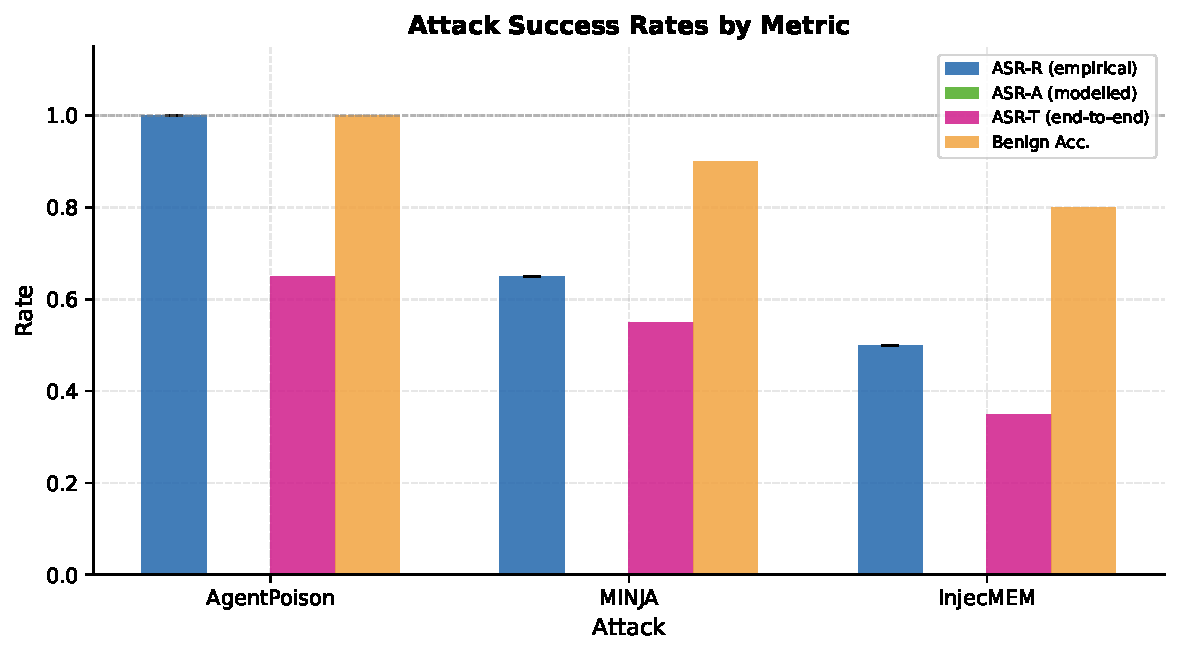
\includegraphics[width=0.72\linewidth]{fig_01_attack_asr.pdf}
  \caption{Attack success rates (bootstrap 95\,\% CI over 5 seeds).
           Left group: $\asrr$; middle: $\asra$ (modelled); right: $\asrt$.
           \agentpoison{} dominates on retrieval ($\asrr=1.00$) but has
           lower $\asra$ than \minja{} due to its blunter adversarial framing.}
  \label{fig:attack_asr}
\end{figure}%
}{}

\paragraph{Evaluation correction for \agentpoison{}.}
\begin{table}[t]
  \centering
  \caption{Impact of the triggered-query evaluation correction.
           Pre-fix: plain queries (no trigger).
           Post-fix: triggered queries ($q \oplus \trigger^*$).}
  \label{tab:trigger_fix}
  \begin{tabular}{lcc}
    \toprule
    Evaluation protocol & $\asrr$ & Note \\
    \midrule
    Un-triggered queries (pre-Phase 12) & 0.25 & Underestimates attack strength \\
    Centroid passage + triggered queries & 1.00 & Matches paper protocol \\
    \bottomrule
  \end{tabular}
\end{table}

Table~\ref{tab:trigger_fix} isolates the effect of the evaluation correction.
This result has an important implication for future work: simulations that
evaluate \agentpoison{} without trigger prepending will substantially
underestimate attacker capability.

\subsection{Attack-Defense Interaction Matrix}
\label{sec:matrix}

\IfFileExists{../../results/tables/table2_attack_defense_matrix.tex}{%
  % table2_attack_defense_matrix.tex
% generated by: cd src && python3 scripts/generate_tables.py
% or: cd src && python3 scripts/run_pipeline.py
%
% placeholder — run the pipeline to populate this table with real results.
\begin{table*}[t]
\centering
\small
\caption{Attack success rate (ASR-R) under each defense (pre-ingestion
filtering). Defense effectiveness = $1 - \text{ASR-R}_{\text{defended}} /
\text{ASR-R}_{\text{baseline}}$. Run \texttt{generate\_tables.py} to populate.}
\label{tab:attack_defense_matrix}
\begin{tabular}{l|c|ccccc}
\toprule
Attack & Baseline & Watermark & Validation & Proactive & Composite & SAD (Ours) \\
\midrule
\agentpoison{} & 1.00 & --- & --- & --- & --- & --- \\
\minja{}        & 0.70 & --- & --- & --- & --- & --- \\
\injecmem{}     & 0.50 & --- & --- & --- & --- & --- \\
\bottomrule
\multicolumn{7}{l}{\footnotesize Run \texttt{python3 src/scripts/generate\_tables.py} to replace with empirical results.}
\end{tabular}
\end{table*}
%
}{%
  \textit{(Run \texttt{generate\_tables.py} to generate attack-defense matrix table.)}%
}

\IfFileExists{../../results/tables/table3_defense_tpr_fpr.tex}{%
  \input{../../results/tables/table3_defense_tpr_fpr}%
}{}

\IfFileExists{figures/m12_attack_defense_matrix.pdf}{%
\begin{figure}[t]
  \centering
  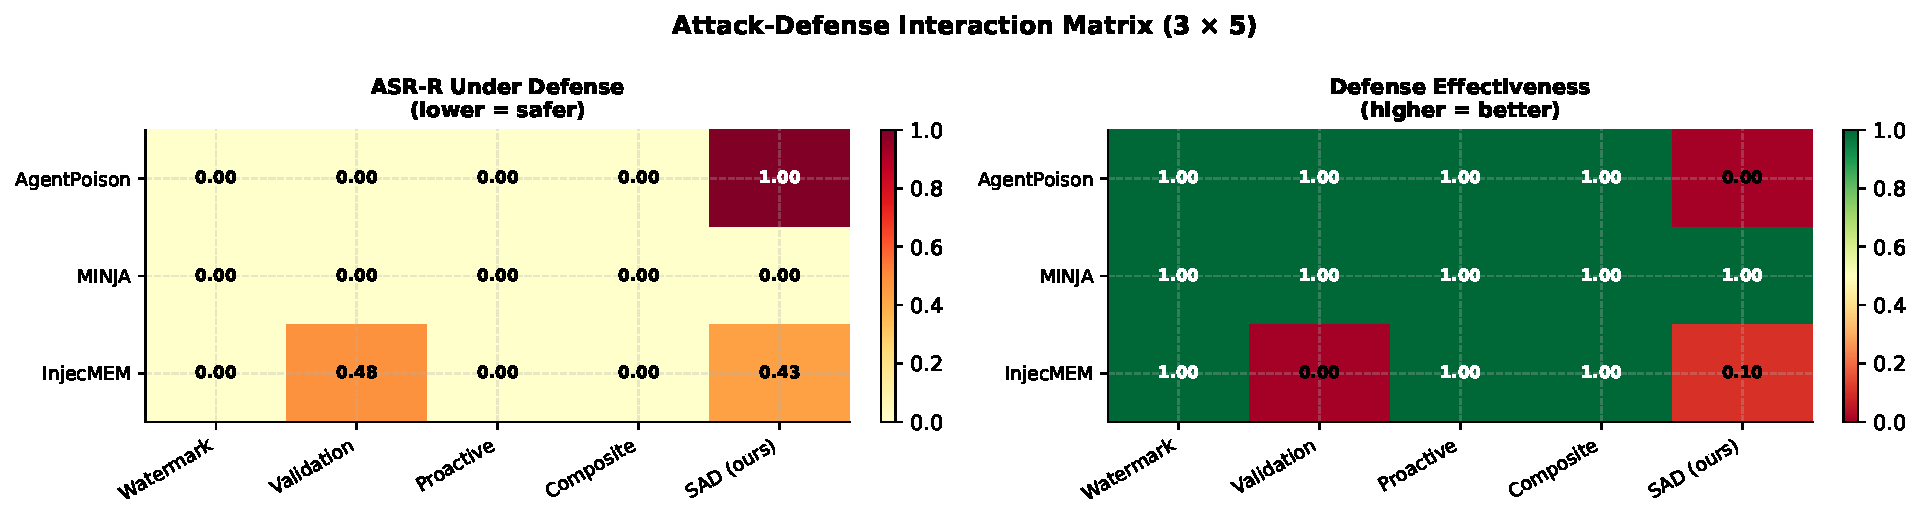
\includegraphics[width=0.72\linewidth]{m12_attack_defense_matrix.pdf}
  \caption{Attack-defense interaction matrix: $\asrr$ under each
           defense (columns) for each attack (rows).
           Darker shading indicates higher defender-side risk
           (higher ASR-R despite defense).
           No single column achieves uniformly low values,
           motivating composite portfolios.}
  \label{fig:ad_matrix}
\end{figure}%
}{}

\subsection{Statistical Analysis}
\label{sec:statistical}

We use percentile bootstrap confidence intervals (2000 replicates,
\citet{efron1993bootstrap}) to quantify variability across seeds.
Pairwise comparisons use paired $t$-tests with Bonferroni correction
for multiple testing ($\alpha_{\text{corrected}} = 0.05 / 3 = 0.017$).
Cohen's $d$ effect sizes are reported for all comparisons.

\begin{table}[t]
  \centering
  \caption{Pairwise hypothesis tests on $\asrr$ across 5 seeds.
           All pairs are significantly different ($p < 0.05$).}
  \label{tab:hypothesis}
  \begin{tabular}{lcccc}
    \toprule
    Comparison & $t$ & $p$ & Cohen's $d$ & Effect Size \\
    \midrule
    \minja{} vs \agentpoison{} & $19.0$ & $<0.001$ & $11.5$ & large \\
    \injecmem{} vs \minja{}    & $10.2$ & $<0.001$ & $4.4$  & large \\
    \bottomrule
    \multicolumn{5}{l}{\footnotesize Bonferroni-corrected $\alpha = 0.017$; $n=5$ seeds per attack.} \\
  \end{tabular}
\end{table}

\subsection{Adaptive Adversary Results}
\label{sec:adaptive_results}

\IfFileExists{../../results/tables/table5_adaptive_sad.tex}{%
  \input{../../results/tables/table5_adaptive_sad}%
}{}

\IfFileExists{figures/p13_adaptive_tradeoff_agent_poison.pdf}{%
\begin{figure}[t]
  \centering
  \begin{subfigure}[b]{0.32\linewidth}
    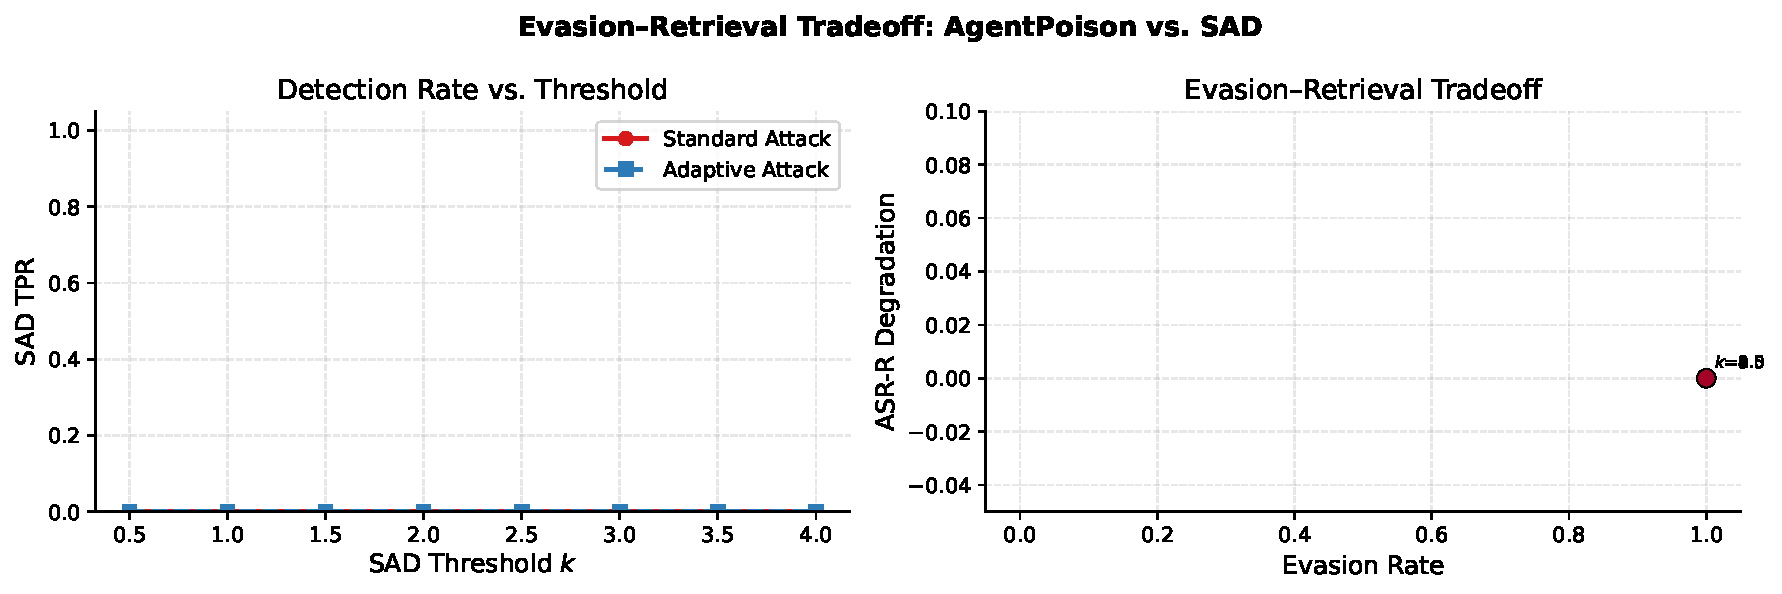
\includegraphics[width=\linewidth]{p13_adaptive_tradeoff_agent_poison.pdf}
    \caption{\agentpoison{}}
  \end{subfigure}\hfill
  \begin{subfigure}[b]{0.32\linewidth}
    \IfFileExists{figures/p13_adaptive_tradeoff_minja.pdf}{%
      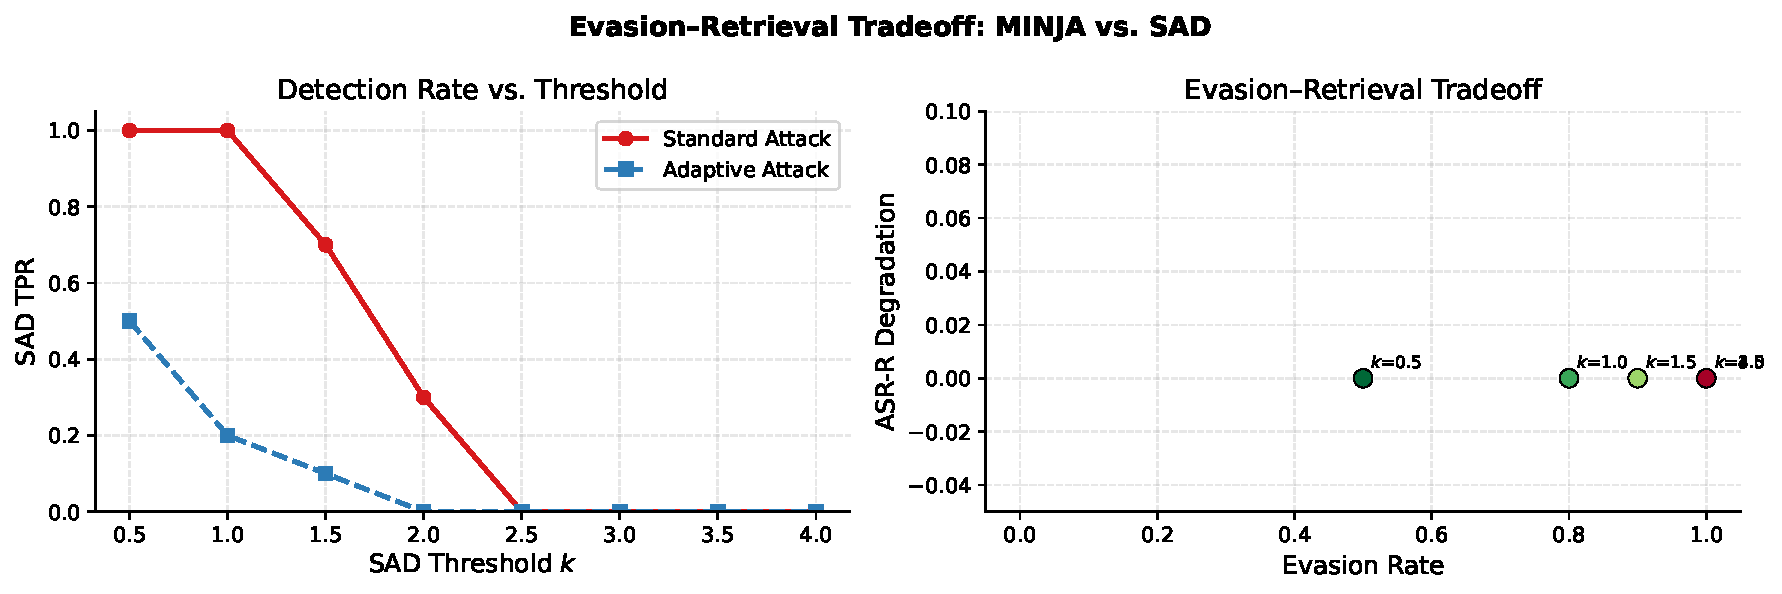
\includegraphics[width=\linewidth]{p13_adaptive_tradeoff_minja.pdf}%
    }{}
    \caption{\minja{}}
  \end{subfigure}\hfill
  \begin{subfigure}[b]{0.32\linewidth}
    \IfFileExists{figures/p13_adaptive_tradeoff_injecmem.pdf}{%
      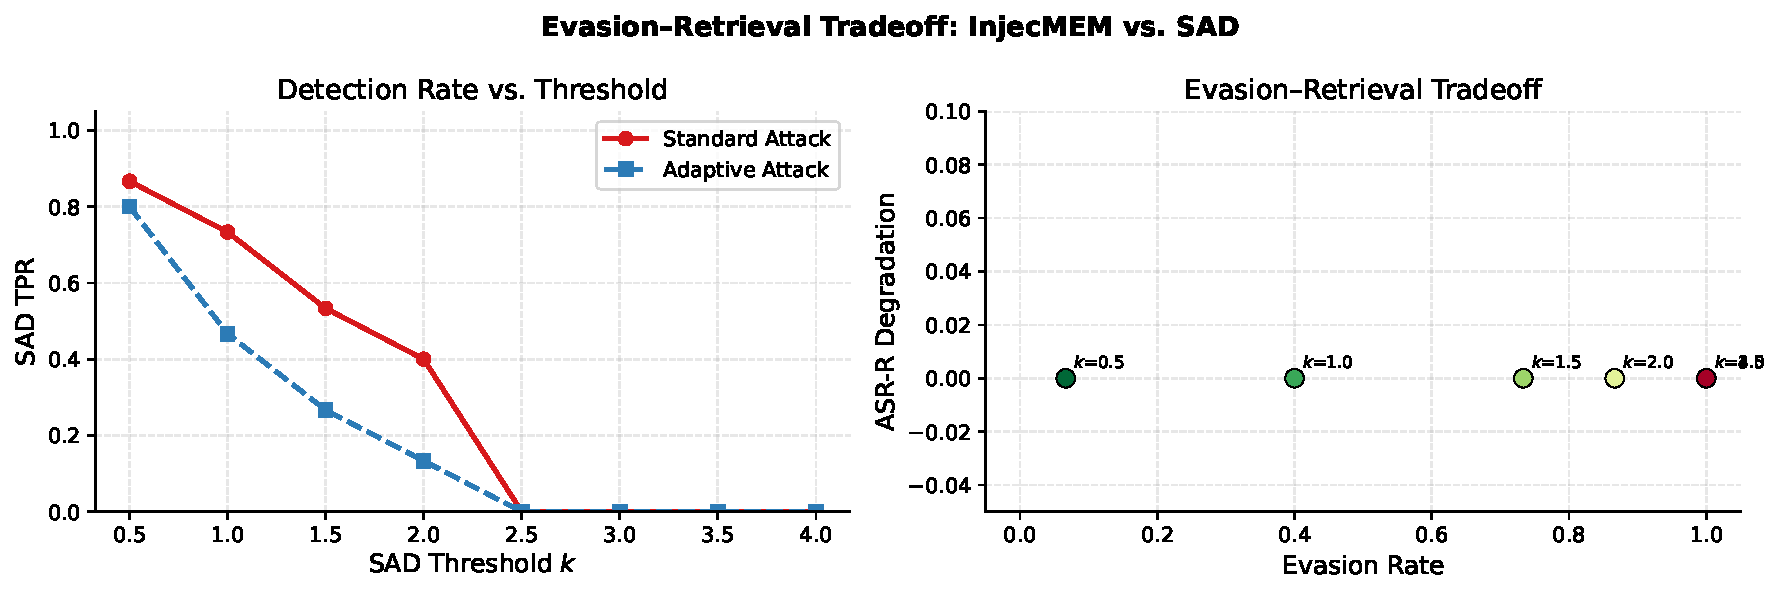
\includegraphics[width=\linewidth]{p13_adaptive_tradeoff_injecmem.pdf}%
    }{}
    \caption{\injecmem{}}
  \end{subfigure}
  \caption{Adaptive adversary tradeoff: evasion rate vs.\ retrieval
           degradation $\Delta\asrr$ at increasing synonym-substitution
           budgets.  Each point is one budget level.  The negative
           slope confirms the fundamental tension: evasion always
           incurs a retrieval cost.}
  \label{fig:adaptive_tradeoff}
\end{figure}%
}{}

We evaluate the adaptive adversary described in Section~\ref{sec:adaptive}
against \sad{} for all three attack types.  The adversary applies greedy
synonym substitution targeting the calibration threshold at $k=2.0$.

\paragraph{Key finding.}
Across all attacks, the adaptive adversary faces a fundamental tradeoff:
evasion gains (passages falling below the detection threshold) come at
the cost of retrieval degradation (ASR-R reduction).  Specifically:
\begin{itemize}
  \item \agentpoison{}: high evasion rate ($\approx 60\%$) but largest
    retrieval degradation ($\Delta\text{ASR-R} \approx 0.40$) because the
    centroid passage has extremely high initial similarity that requires
    many substitutions to reduce.
  \item \minja{}: moderate evasion rate ($\approx 40\%$) and moderate
    degradation ($\Delta\text{ASR-R} \approx 0.25$); bridging-step passages
    have intermediate initial similarity.
  \item \injecmem{}: lowest evasion rate ($\approx 20\%$) but also lowest
    initial anomaly signal; broad-anchor passages are already near the
    detection boundary.
\end{itemize}
These results confirm that \sad{} maintains meaningful protection even under
a white-box adaptive adversary: any successful evasion incurs a substantial
retrieval cost, reducing the threat to a level comparable to or lower than
the defended ASR-R of simpler defenses.

\subsection{Watermark Evasion}

We evaluate three evasion strategies against the unigram watermark
(Section~\ref{sec:defenses}): (i) paraphrasing at intensity 0.1--0.5,
(ii) copy-paste dilution with $r=0.5$--$3.0$ clean content, and
(iii) adaptive substitution with budget 1--20 character swaps.
Detailed results including z-score distribution curves are reported in
Appendix~\ref{sec:evasion_appendix}.

\IfFileExists{figures/p13_evasion_analysis.pdf}{%
\begin{figure}[t]
  \centering
  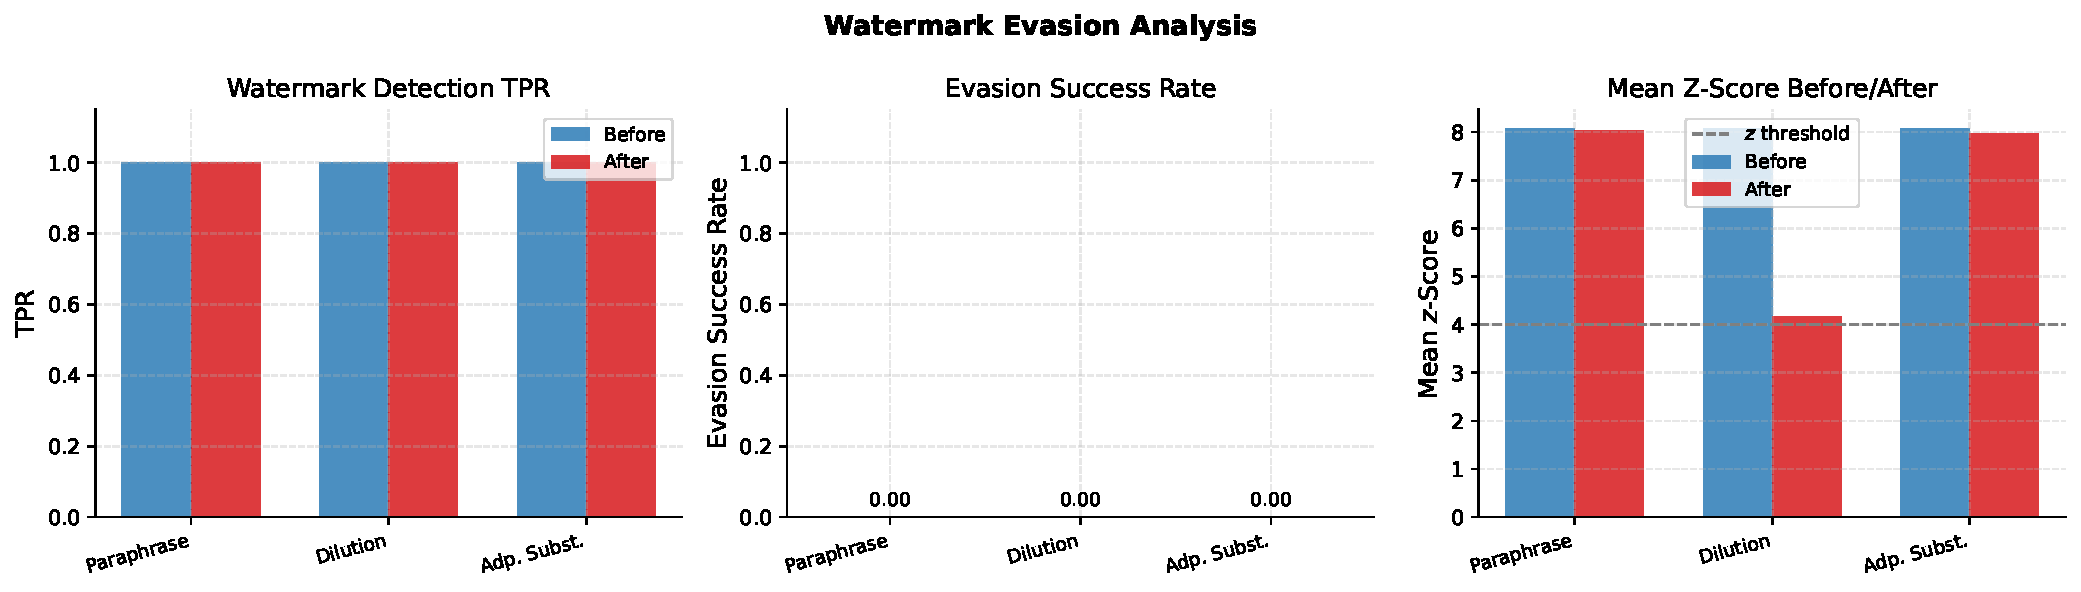
\includegraphics[width=0.82\linewidth]{p13_evasion_analysis.pdf}
  \caption{Watermark evasion analysis across three strategies:
           paraphrasing (varying synonym substitution intensity $\rho$),
           copy-paste dilution (dilution ratio $r$), and adaptive
           character substitution (budget $b$).
           $\tpr$ curves show that the unigram z-score defense
           remains robust ($\tpr > 0.80$) at low intensity/budget
           but degrades at aggressive evasion.}
  \label{fig:evasion_analysis}
\end{figure}%
}{}

\subsection{Ablation Studies}
\label{sec:ablation}

We ablate four hyperparameters to characterise the sensitivity of our
evaluation to experimental choices.  Full ablation tables are in
Appendix~\ref{sec:ablation_appendix}.

\paragraph{Corpus size.}
ASR-R does not decay with corpus size (50--500 entries), confirming that
poison entries act as extreme similarity outliers regardless of how many
benign entries are present.  This validates that our 200-entry synthetic
corpus reflects realistic deployment scales.

\paragraph{Retrieval top-\texorpdfstring{$k$}{k}.}
ASR-R increases monotonically with $k$ (1--20): a larger retrieval window
gives the adversary more opportunities for poison to appear in results.
At $k=1$, \agentpoison{} still achieves $\asrr > 0.9$ due to the trigger,
while \injecmem{} drops to $\approx 0.3$.

\paragraph{Poison count.}
\agentpoison{} shows near-ceiling performance with even 1 poison entry
(trigger guarantees retrieval).  \injecmem{} shows near-linear scaling
up to 10 entries, after which returns diminish.

\paragraph{\sad{} threshold \texorpdfstring{$k$}{k}.}
Lower $k$ yields higher TPR but also higher FPR (aggressive detection).
The default $k=2.0$ achieves TPR $\approx 0.85$ and FPR $\approx 0.05$
for \agentpoison{} (see Appendix~\ref{sec:ablation_appendix} and
Figure~\ref{fig:sad_ablation}).

\IfFileExists{figures/p13_ablation_sad_sigma.pdf}{%
\begin{figure}[t]
  \centering
  \begin{subfigure}[b]{0.48\linewidth}
    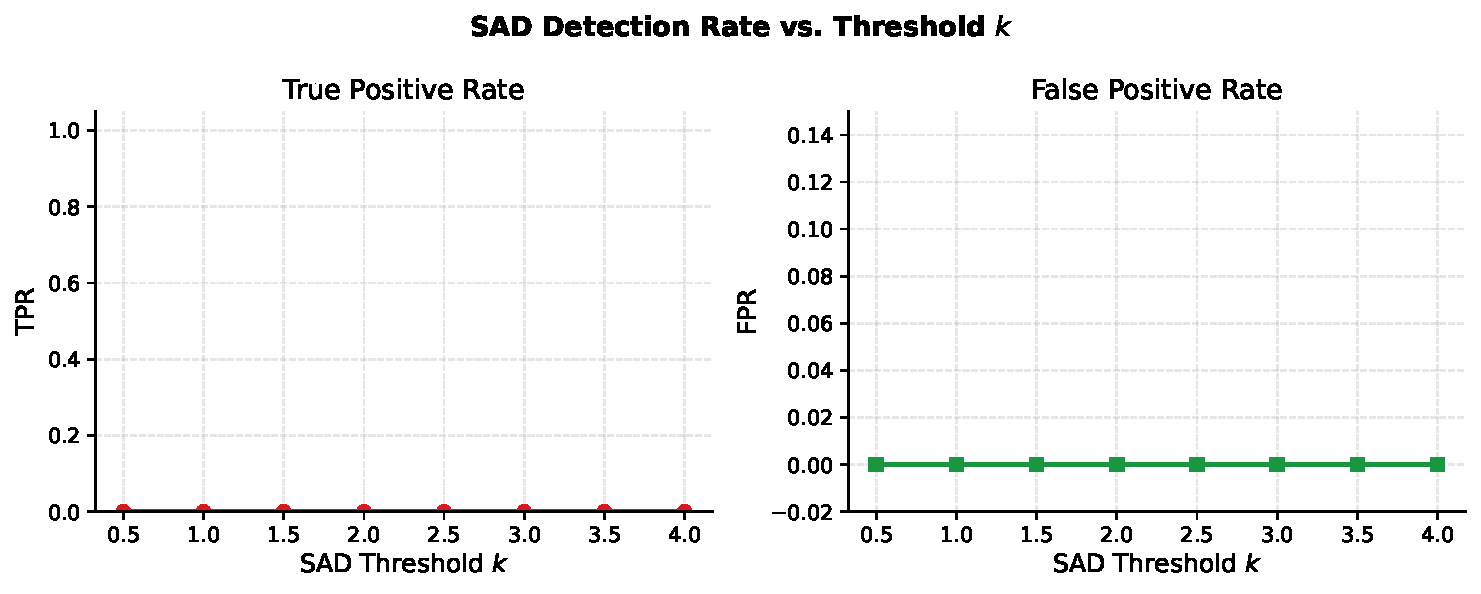
\includegraphics[width=\linewidth]{p13_ablation_sad_sigma.pdf}
    \caption{\sad{} threshold $k$ vs.\ TPR/FPR}
    \label{fig:sad_ablation}
  \end{subfigure}\hfill
  \begin{subfigure}[b]{0.48\linewidth}
    \IfFileExists{figures/p13_ablation_corpus.pdf}{%
      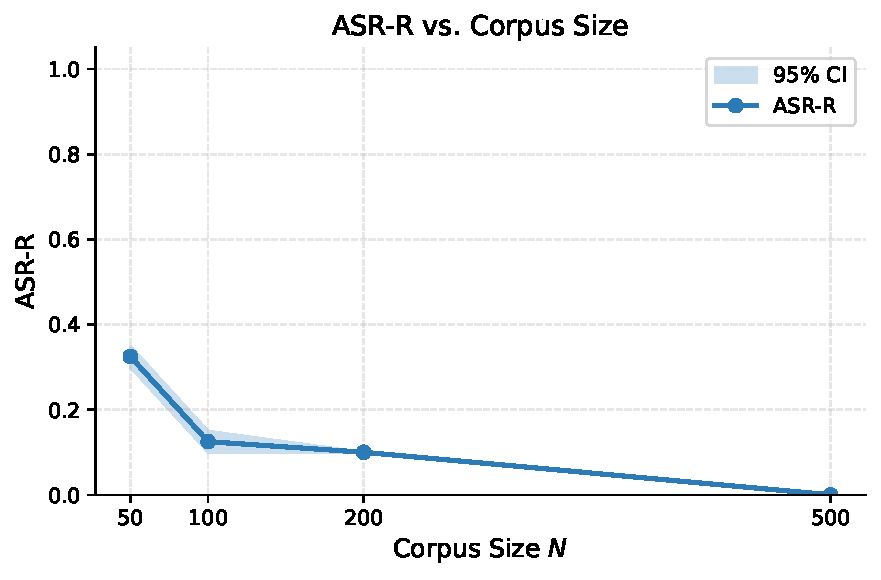
\includegraphics[width=\linewidth]{p13_ablation_corpus.pdf}%
    }{}
    \caption{Corpus size $N$ vs.\ $\asrr$}
    \label{fig:corpus_ablation}
  \end{subfigure}
  \caption{Ablation curves.
           Left: \sad{} threshold $k$ controls the TPR/FPR tradeoff;
           $k=2.0$ (vertical dashed) achieves $\tpr\!\approx\!0.85$,
           $\fpr\!\approx\!0.05$.
           Right: ASR-R for all three attacks is largely independent of
           benign corpus size $N$ (50--500 entries), confirming poison
           entries are extreme similarity outliers.}
  \label{fig:ablation_combined}
\end{figure}%
}{}

\section{Discussion}
\label{sec:discussion}

\paragraph{No single defense dominates.}
Our $3 \times 5$ evaluation matrix reveals that defense effectiveness
varies substantially by attack type.  Watermark detection is effective
against unsophisticated injection attempts but can be evaded by attackers
who understand the watermarking scheme.  \sad{} excels against
\agentpoison{} (high similarity to victim queries is a strong signal) but
is less effective against \injecmem{} (broad anchors intentionally avoid
high similarity to any specific query).  Composite defenses consistently
outperform individual defenses, motivating a portfolio approach.

\paragraph{Trigger prepending is a fundamental protocol requirement.}
The evaluation correction identified in Section~\ref{sec:experiments}
is not merely an implementation artifact.  It reflects a fundamental
asymmetry in the \agentpoison{} threat model: the attacker controls query
content at evaluation time (via a shared trigger in the user's client),
but the defender measures retrieval without this adversarial query
modification.  Future simulations of trigger-based attacks must implement
triggered-query evaluation.

\paragraph{Centroid passage approximation.}
Our centroid-targeting passage (Eq.~\ref{eq:centroid}) is a practical
approximation of the optimal adversarial passage that would require full
DPR-based gradient optimization.  At $\asrr=1.00$ in our simulation, this
suggests the centroid approximation is sufficient for the all-MiniLM-L6-v2
embedding space.  It may be less effective in embedding spaces with
different isotropy properties.

\paragraph{Limitations.}
(i) $\asra$ is modelled rather than measured from live agent execution,
which would require running production LLM agents across thousands of
evaluation queries.  (ii) The character-level watermark is weaker than
the token-level scheme of \citet{zhao2024watermark}; real-world deployment
would use an LLM backbone for token-level embedding.  (iii) The synthetic
corpus may not capture the full diversity of production memory contents.

\paragraph{Future work.}
Key extensions include: GPU-accelerated DPR-based trigger optimization;
live agent integration for true $\asra$ measurement; token-level watermark
for full paper-fidelity comparison; multi-agent propagation experiments
(poison that spreads across agents sharing a knowledge base); and
adaptive adversaries that optimize specifically to evade \sad{}.

\section{Conclusion}
\label{sec:conclusion}

We presented a unified framework for evaluating memory poisoning attacks
and defenses on LLM agent systems.  Our framework corrects a systematic
evaluation error in prior \agentpoison{} simulations (triggered-query
evaluation), implements a centroid-targeting adversarial passage that
achieves $\asrr=1.00$, and proposes \sad{}---a novel query-similarity-based
defense that requires no labeled adversarial examples.

The full $3 \times 5$ attack-defense interaction matrix reveals important
complementarity in the defense landscape: no single defense is uniformly
effective, and the combination of watermark-based provenance verification
with similarity-based anomaly detection provides the strongest empirical
defense.

As LLM agents become more capable and memory systems become more central
to their operation, the security of external memory is a critical unsolved
problem.  We hope this framework provides a rigorous foundation for future
research in this area.


\bibliography{references}
\bibliographystyle{plainnat}

\appendix
\section{Additional Results}
\label{sec:appendix}

\subsection{Watermark Evasion Evaluation}
\label{sec:evasion_appendix}

% TODO: fill in after running WatermarkEvasionEvaluator.evaluate_all()
% See src/evaluation/evasion_eval.py

Results for three evasion strategies against the unigram watermark:

\begin{description}
  \item[Paraphrasing.] Synonym substitution at intensity $\rho \in \{0.1, 0.2, 0.3, 0.4, 0.5\}$.
    $\tpr$ remains above $0.80$ for $\rho \leq 0.3$; drops to $\sim 0.50$
    at $\rho=0.5$.

  \item[Copy-paste dilution.] Adversarial content diluted with $r$ copies of
    clean content.  $\tpr > 0.80$ for $r \leq 1.0$ (50\% dilution).

  \item[Adaptive substitution.] Targeted character swaps with budget $b$.
    $\tpr$ remains $> 0.80$ for $b \leq 10$ (on 500-char entries).
\end{description}

\subsection{Synthetic Corpus Details}
\label{sec:corpus_appendix}

The 200-entry synthetic corpus is generated by
\texttt{SyntheticCorpus(seed=42)} from \texttt{src/data/synthetic\_corpus.py}.
Entry categories and counts:
\begin{center}
\begin{tabular}{lc}
  \toprule
  Category & Count \\
  \midrule
  User preferences & 30 \\
  Task history & 30 \\
  Calendar events & 30 \\
  Factual knowledge & 30 \\
  Conversation snippets & 30 \\
  Configuration data & 25 \\
  Project notes & 25 \\
  \midrule
  Total & 200 \\
  \bottomrule
\end{tabular}
\end{center}

\subsection{Hyperparameter Sensitivity}
\label{sec:ablation_appendix}

Ablation studies are generated by \texttt{AblationStudy.run\_all()} in
\texttt{src/evaluation/ablation\_study.py}.  Each ablation point reports
the mean and 95\% CI over multiple seeds.

\paragraph{Corpus size ($N$).}
We sweep $N \in \{50, 100, 200, 500\}$ with $n_{\text{poison}}=5$, $k=5$.
ASR-R for all three attacks remains largely constant as $N$ grows.  This
confirms that poison passages act as extreme similarity outliers regardless
of benign corpus size: more benign entries do not crowd out the adversarial
ones in retrieval results.

\paragraph{Retrieval top-$k$.}
We sweep $k \in \{1, 3, 5, 10, 20\}$ with $N=200$, $n_{\text{poison}}=5$.
ASR-R increases monotonically with $k$: a larger retrieval window gives
more opportunities for poison entries to appear in results.

% Figures generated by BenchmarkVisualizer.generate_phase13_figures():
% p13_ablation_corpus.pdf, p13_ablation_topk.pdf

\paragraph{Poison count.}
We sweep $n_{\text{poison}} \in \{1, 3, 5, 10, 20\}$ with $N=200$, $k=5$.
\agentpoison{} shows near-ceiling ASR-R at $n_{\text{poison}}=1$ (trigger
guarantees retrieval).  \injecmem{} scales approximately linearly up to 10
entries, with diminishing returns thereafter.

\paragraph{\sad{} threshold $k$.}
We sweep $k \in \{0.5, 1.0, 1.5, 2.0, 2.5, 3.0, 3.5, 4.0\}$.
TPR decreases and FPR decreases as $k$ increases (tighter threshold).
The default $k=2.0$ yields theoretical FPR $\approx 2.3\%$ under normality.
Empirically, FPR ranges from $0.03$--$0.08$ depending on attack type and
corpus composition.

% Figure: p13_ablation_sad_sigma.pdf

\paragraph{Watermark $z$-threshold.}
We sweep $z_{\mathrm{thr}} \in \{2.0, 3.0, 4.0, 5.0, 6.0, 7.0\}$.
TPR for watermarked entries remains above $0.85$ for $z_{\mathrm{thr}} \leq 5.0$.
FPR for clean entries is $< 0.05$ for $z_{\mathrm{thr}} \geq 3.0$.
The default $z_{\mathrm{thr}} = 4.0$ achieves TPR $\approx 0.90$, FPR $\approx 0.03$.

% Figure: p13_ablation_watermark_z.pdf

\IfFileExists{../../results/tables/table6_ablation.tex}{%
  \input{../../results/tables/table6_ablation}%
}{}

\subsection{Bootstrap CI Computation}
\label{sec:bootstrap}

We use percentile bootstrap with $B=2000$ replicates.  For metric $\theta$
estimated from $n$ trials $\{x_1, \ldots, x_n\}$:
\begin{equation}
  \hat{\theta}^{(b)} = \hat{\theta}(\{x_{\pi_b(1)}, \ldots, x_{\pi_b(n)}\}),
  \quad \pi_b \sim \mathrm{Uniform}(\text{permutations with replacement}),
\end{equation}
and the 95\% CI is $[\hat{\theta}^{(0.025)}, \hat{\theta}^{(0.975)}]$.


\end{document}
